\documentclass[12pt]{article}

\usepackage{hyperref,graphicx}
\usepackage{fullpage}

\title{Half Field Offense \\ Technical Manual}
\author{Matthew Hausknecht}

\begin{document}

\maketitle
\tableofcontents

\section{Overview}

This document describes the state and action spaces of the HFO domain.

\section{State Spaces}

The HFO domains provides a choice between a low-level feature set and
a higher-level feature set. Selecting between the different feature
sets is accomplished when connecting to the agent server. See
\verb|examples/hfo_example_agent.cpp| and 
\verb|examples/hfo_example_agent.py| for examples.

\subsection{High Level Feature Set}
A set of high-level features is provided following the example given
by Barrett et al. pp. 159-160 \cite{THESIS14-Barrett}. Barrett writes
``There are many ways to represent the state of a game of half field
offense.  Ideally, we want a compact representation that allows the
agent to learn quickly by generalizing its knowledge about a state to
similar states without over-constraining the policy.'' All features
are encoded a floating point values and normalized to the range of
[-1,1]. Invalid features are given a value of -2. The features are as
follows:

\subsubsection{High Level State Feature List}
\begin{itemize}
\item{\textbf{X position} - The agent’s x position on the field.}
\item{\textbf{Y position} - The agent’s y position on the field.}
\item{\textbf{Orientation} - The direction that the agent is facing.}
\item{\textbf{Ball Distance} - Distance to the ball.}
\item{\textbf{Ball Angle} - Angle to the ball.}
\item{\textbf{Able to Kick} - Boolean indicating if the agent can kick the ball.}
\item{\textbf{Goal Center Distance} - Distance from the agent to the center of the goal.}
\item{\textbf{Goal Center Angle} - Angle from the agent to the center of the goal.}
\item{\textbf{Goal opening angle} - The size of the largest open angle
  of the agent to the goal, shown as $\theta_g$ in Figure
  \ref{fig:openAngle}.}
\item{\textbf{Teammate i's goal opening angle} - For each teammate i:
  the i’s goal opening angle}
\item{\textbf{Distance to Opponent} - If an opponent is present,
  distance to the closest opponent. This feature is absent if there
  are no opponents.}
\item{\textbf{Distance from teammate i to opponent} - For each
  teammate i: the distance from the teammate to the closest
  opponent. This feature is absent if there are no opponents. If
  teammates are present but not detected, this feature is considered
  invalid and given the value of -2.}
\item{\textbf{Pass opening angle i} - For each teammate i: the open
  angle available to pass to teammate i. Shown as $\theta_p$ in Figure
  \ref{fig:openAngle}. If teammates are present but not detected, this
  feature is considered invalid and given the value of -2.}
\end{itemize}

\begin{figure}[htp]
  \centering
  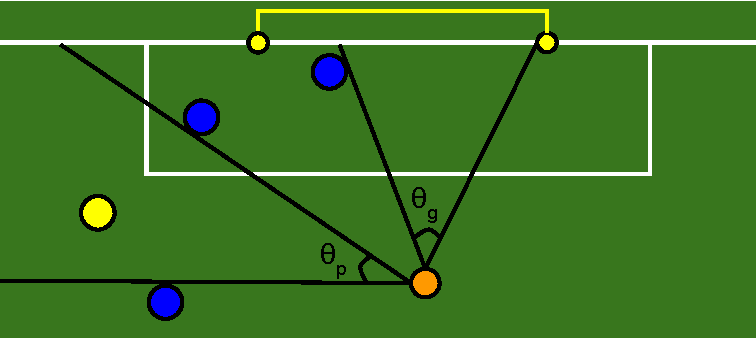
\includegraphics[width=.75\textwidth]{figures/openAngle}
  \caption{Open angle from ball to the goal $\theta_g$ avoiding the
    blue goalie and the open angle from the ball to the yellow
    teammate $\theta_p$. Figure reproduced with permission from Samuel
    Barrett.}
  \label{fig:openAngle}
\end{figure}

\subsection {Low Level Feature Set}
The state features used by HFO are designed with the mindset of
providing an overcomplete, basic, egocentric viewpoint. The features
are basic in the sense that they provide distances and angles to
relevant points of interest, but do not include higher level
perceptions such as the largest angle between a goal post and
goalkeeper.

All features are encoded as floating point values normalized to the
range of [-1,1]. Different types of features are discussed next.

\subsubsection{Boolean Features}

Boolean features assume either the minimum feature value of -1 or the
maximum feature value of 1.

\subsubsection{Valid Features}

Since feature information is attained from the Agent's world-model, it
is possible that, the world model's information may be stale or
incorrect. \textit{Valid features} are boolean features indicating
consistency of world model predictions. For example, if the world
model's estimate of the agent's position is known to be flawed, the
\textit{valid feature} for self position would assume the minimum
value of -1. Otherwise it will assume the maximum value of 1.

The features associated with a valid feature are given the value of
zero if an inconsistency is detected. For example, if the world model
detects that the agent's velocity is invalid, the feature that encodes
the magnitude of self velocity will be set to zero.

\subsubsection{Angular Features}

\textit{Angular features} (e.g. the angle to the ball), are encoded as two
floating point numbers -- the $sin(\theta)$ and $cos(\theta)$ where
$\theta$ is the original angle.

This encoding allows the angle to vary smoothly for all possible
angular values. Other encodings such as radians or degrees have a
discontinuity that when normalized, could cause the feature value to
flip between the maximum and minimum value in response to small
changes in $\theta$.

\subsubsection{Distance Features}

\textit{Distance features} encode the distance to objects of
interest. Unless otherwise indicated, they are normalized against the
maximum possible distance in the HFO playfield (defined as $\sqrt{l^2
  + w^2}$ where $l,w$ are the length and width of the HFO
playfield). A distance of zero will be encoded with the minimum
feature value of -1 while a maximum distance will be encoded with 1.

\subsubsection{Landmark Features}

Landmark features encode the relative angle and distance to a landmark
of interest. Each landmark feature consists of three floating point
values, two to encode the angle to the landmark and one to encode the
distance. Note that if the agent's self position is invalid, then the
landmark feature values are zeroed.

\subsubsection{Player Features}

Player features are used to encode the relationship of the agent to
another player or opponent. Each player feature is encoded as 1) a
landmark feature of that player's location 2) the global angle of that
player's body 3) the magnitude of the player's velocity and 4) the
global angle of the player's velocity. Eight floating point numbers
are used to encode each player feature.

\subsubsection{Other Features}

Some features, such as the agent's stamina, do not fall into any of
the above categories. These features are referred to as \textit{other
  features}.

\subsubsection{Low Level State Feature List}

Basic Features are always present and independent of the number of
teammates or opponents. The 32 basic features are encoded using 58
floating point values (\textit{angular features} require two floats,
\textit{landmark features} require 3). Additionally a variable number
of \textit{player features} are then added. This number depends on the
number of teammates and opponents in the HFO game, but 8 floating
point values are required for each player feature. Thus, the total
number of features is $58 + 8*\textrm{num\_teammates} +
8*\textrm{num\_opponents}$.

\begin{itemize}
  \item{\textbf{Self\_Pos\_Valid} [Valid] Indicates if self position is valid.}
  \item{\textbf{Self\_Vel\_Valid} [Valid] Indicates if the agent's velocity is valid.}
  \item{\textbf{Self\_Vel\_Ang} [Angle] Angle of agent's velocity.}
  \item{\textbf{Self\_Vel\_Mag} [Other] Magnitude of agent's
    velocity. Normalized against the maximum observed self speed,
    0.46.}
  \item{\textbf{Self\_Ang} [Angle] Agent's Global Body Angle.}
  \item{\textbf{Stamina} [Other] Agent's Stamina: The amount of remaining stamina the
    agent has. Normalized against the maximum observed agent stamina
    of 8000.}
  \item{\textbf{Frozen} [Boolean] Indicates if the agent is Frozen. Frozen status can
    happen when being tackled by another player.}
  \item{\textbf{Colliding\_with\_ball} [Boolean] Indicates if the agent
    is colliding with the ball.}
  \item{\textbf{Colliding\_with\_player} [Boolean] Indicates if the agent
    is colliding with another player.}
  \item{\textbf{Colliding\_with\_post} [Boolean] Indicates if the agent
    is colliding with a goal post.}
  \item{\textbf{Kickable} [Boolean] Indicates if the agent is able to
    kick the ball.}
  \item{\textbf{Goal Center} [Landmark] Center point between the goal posts.}
  \item{\textbf{Goal Post Top} [Landmark] Top goal post.}
  \item{\textbf{Goal Post Bot} [Landmark] Bottom goal post.}
  \item{\textbf{Penalty Box Center} [Landmark] Center of the penalty box line.}
  \item{\textbf{Penalty Box Top} [Landmark] Top corner of the penalty box.}
  \item{\textbf{Penalty Box Bot} [Landmark] Bottom corner of the penalty box.}
  \item{\textbf{Center Field} [Landmark] The left middle point of the
    HFO play area. True center of the full-field.}
  \item{\textbf{Corner Top Left} [Landmark] Top left corner HFO Playfield.}
  \item{\textbf{Corner Top Right} [Landmark] Top right corner HFO Playfield.}
  \item{\textbf{Corner Bot Right} [Landmark] Bot right corner HFO Playfield.}
  \item{\textbf{Corner Bot Left} [Landmark] Bot left corner HFO Playfield.}
  \item{\textbf{OOB Left Dist} [Distance] Distance to the nearest
    point of the left side of the HFO playable area. E.g. distance
    remaining before the agent goes out of bounds in left field.}
  \item{\textbf{OOB Right Dist} [Distance] Distance remaining before
    the agent goes out of bounds in right field.}
  \item{\textbf{OOB Top Dist} [Distance] Distance remaining before
    the agent goes out of bounds in top field.}
  \item{\textbf{OOB Bot Dist} [Distance] Distance remaining before
    the agent goes out of bounds in bottom field.}
  \item{\textbf{Ball Pos Valid} [Valid] Indicates if the ball position estimate is valid.}
  \item{\textbf{Ball Angle} [Angle] Angle to the ball from the agent's perspective.}
  \item{\textbf{Ball Dist} [Distance] Distance to the ball.}
  \item{\textbf{Ball Vel Valid} [Valid] Indicates if the ball velocity estimate is valid.}
  \item{\textbf{Ball Vel Mag} [Other] Global magnitude of the ball velocity. Normalized against the observed maximum ball velocity, 3.0.}
  \item{\textbf{Ball Vel Ang} [Angle] Global angle of ball velocity.}
  \item{\textbf{Teammate Features} [Player] One teammate feature for each teammate active in HFO, sorted by proximity to the agent.}
  \item{\textbf{Opponent Features} [Player] One opponent feature for each opponent present, sorted by proximity to the player.}
\end{itemize}

\section{Action Space}
The HFO domain provides support for both low-level primitive actions
and high-level strategic actions. Basic, parameterized actions are
provided for locomotion and kicking. Additionally high-level strategic
actions are available for moving, shooting, passing and
dribbling. Control of the agent's head and gaze is not provided and
follows Agent2D's default strategy. Selection between high-level and
low-level actions spaces is performed when connecting to the agent
server.

\subsection{Low Level Actions}
\begin{itemize}
\item{\textbf{Dash}(power, degrees): Moves the agent with power [-100,
    100] where negative values move backwards. The relative direction
  of movement is given in degrees and varies between [-180,180] with 0
  degrees being a forward dash and 90 degrees dashing to the agent's
  right side. Note, dashing does not turn the agent.}
\item{\textbf{Turn}(degrees): Turns the agent in the
  specified direction. Valid values range between [-180, 180] degrees
  where 90 degrees turns the agent to directly to its right side.}
\item{\textbf{Tackle}(degrees): Contest the ball. Direction
  varies between [-180, 180]. TODO: Better description.}
\item{\textbf{Kick}(power, degrees): Kick the ball with power [0, 100]
  in relative direction [-180, 180]. Has no effect if the agent does
  not possess the ball.}
\item{\textbf{Quit}: Indicates to the agent server that you wish to
  terminate the HFO environment.}
\end{itemize}

\subsection{High Level Actions}
\begin{itemize}
\item{\textbf{Move}(): Re-positions the agent according to the
  strategy given by Agent2D. The \textit{move} command works only when
  agent does not have the ball. If the agent has the ball, another
  command such as \textit{dribble}, \textit{shoot}, or \textit{pass}
  should be used.}
\item{\textbf{Shoot}(): Executes the best available shot. This command
  only works when the agent has the ball.}
\item{\textbf{Pass}(): Finds the best teammate to pass to and the type
  of pass to use. This command only works when the agent has the
  ball.}
\item{\textbf{Dribble}(): Advances the ball towards the goal using a
  combination of short kicks and moves.}
\end{itemize}

\bibliographystyle{abbrv}
\bibliography{manual}

\end{document}
